\documentclass[12pt,a4paper]{article}
\usepackage{graphicx}
\usepackage{amsmath,amssymb}
\usepackage{geometry}
\usepackage{cite}
\geometry{left=2.5cm,right=2.5cm,top=2.5cm,bottom=2.5cm}
\usepackage{subcaption}
\usepackage{hyperref}
\usepackage{enumitem}
\usepackage{float}
\usepackage{booktabs}
\usepackage{xcolor}
\usepackage{colortbl}
\usepackage{fancyhdr}
\usepackage{titlesec}

\definecolor{themeblue}{RGB}{41, 65, 122}
\definecolor{lightgray}{gray}{0.92}

\titleformat{\section}{\Large\bfseries\color{themeblue}}{}{0em}{}[\vspace{-0.3cm}\rule{\textwidth}{0.4pt}]
\titleformat{\subsection}{\large\bfseries\color{themeblue!80!black}}{}{0em}{}
\titleformat{\subsubsection}{\normalsize\bfseries\color{themeblue!60!black}}{}{0em}{}

\setlength{\headheight}{14pt}
\pagestyle{fancy}
\fancyhf{}
\fancyhead[C]{\small\color{gray}蒙特卡洛流体仿真实验报告}
\fancyfoot[C]{\thepage}
\renewcommand{\headrulewidth}{0.4pt}
\renewcommand{\footrulewidth}{0pt}

\hypersetup{
    colorlinks=true,
    linkcolor=themeblue!60!black,
    citecolor=themeblue!60!black,
    urlcolor=themeblue!60!black
}

\usepackage{xeCJK}
\setCJKmainfont[AutoFakeBold=3]{SimSun}
\setCJKsansfont[AutoFakeBold=3]{SimHei}
\setCJKmonofont{FangSong}

\title{\vspace{-1cm}\textbf{\LARGE 蒙特卡洛流体仿真实验报告}\\[0.3cm]
\large 2022 涡量法与 2024 速度法的实现与对比}
\author{\textbf{姓名：侍子译} \quad 学号：PB23000284}
\date{\today}

\begin{document}

\maketitle

\begin{abstract}
本实验实现了两种基于 Monte Carlo 的不可压缩流体仿真方法，并进行了定量对比与误差来源分析：
2022 年 Rioux-Lavoie et al. 提出的\textbf{涡量法}\cite{rioux2022}（涡量输运 + Biot-Savart 重建速度）和 2024 年 Sugimoto et al. 提出的\textbf{速度法}\cite{sugimoto2024}（速度算子分裂 + Walk-on-Boundary 投影）。
涡量法以涡量场 $\omega$ 为状态变量，通过 Biot-Savart 积分重建速度，天然满足 $\nabla\cdot\boldsymbol{u}=0$ 且无需投影步骤；速度法以速度场 $\boldsymbol{u}$ 为状态，依赖 WoB 投影维持不可压缩性。
本实验用 CuPy 将 2022 涡量法的核心 Biot-Savart 积分 GPU 化（完美并行负载，加速约 120 倍），并编译运行了 2024 论文的官方实现（VelMCFluids，与论文算法完全一致）。
在粘性 Taylor-Green 涡（$\nu=0.05$，有解析解）基准上进行了定量对比。
结果表明：在 $64\times64$ 网格上，2022 方法的涡量 RMSE（0.51）低于 2024 方法（1.25--0.95），且耗时低约 37 倍（0.13 s vs 4.84 s）。
误差来源分析显示：2022 的误差受限于半拉格朗日平流插值耗散（存在平台约 0.51），而 2024 的误差受限于 WoB 投影的 MC 噪声与投影散度误差（随采样数持续下降但未收敛）。
\end{abstract}

\section{引言}

传统的计算流体力学方法通常依赖网格离散化，在复杂几何边界上面临网格生成困难。近年来，基于随机游走的 Monte Carlo PDE 求解方法——特别是 Walk-on-Spheres（WoS）——被引入流体仿真领域，提供了完全无网格的求解途径。

2022 年，Rioux-Lavoie、Sugimoto 等人提出了首个 Monte Carlo 流体仿真框架\cite{rioux2022}。该方法采用\textbf{涡量-速度}表示：以涡量 $\omega$ 为状态变量，通过 Biot-Savart 定律由涡量重建速度，边界条件通过流函数 $\psi$ 与 WoS 算法处理。由于 Biot-Savart 重建的速度场天然无散，该方法\textbf{无需压力投影}，从根本上避免了不可压缩性约束的数值实现难题。

2024 年，Sugimoto、Batty 和 Hachisuka 提出\textbf{基于速度}的 Monte Carlo 方法\cite{sugimoto2024}。该方法直接以速度场 $\boldsymbol{u}$ 为状态变量，采用经典算子分裂框架（平流→外力→扩散→投影），其中投影步骤用 Walk-on-Boundary（WoB）边界积分直接估计压力梯度 $\nabla p$。由于速度法直接使用速度场，可以方便地融入浮力、PIC/FLIP 等传统速度法技术，但需要显式维持 $\nabla\cdot\boldsymbol{u}=0$。

本实验实现了这两种算法的完整版本：
\begin{itemize}
    \item \textbf{2022 涡量法}：用 CuPy 将 Biot-Savart 积分向量化（\texttt{gpu\_fluid\_2022.py}）；
    \item \textbf{2024 速度法}：编译 2024 论文官方 OptiX 实现（\texttt{VelMCFluids/}）。
\end{itemize}

两者均使用 Numba JIT 加速，在 Taylor-Green 涡流场上从相同初始条件出发进行对比，考察动能演化、涡量守恒和计算效率。

\section{算法原理}

\subsection{2022 涡量法}

\subsubsection{涡量输运方程}

2022 年方法的理论基础是二维不可压缩流的\textbf{涡量输运方程}。对于无粘外流，涡量 $\omega = \partial v/\partial x - \partial u/\partial y$ 沿流线输运：
\begin{equation}
\frac{D\omega}{Dt} = \frac{\partial \omega}{\partial t} + \boldsymbol{u}\cdot\nabla\omega = 0.
\label{eq:vort_transport}
\end{equation}

采用半拉格朗日后向追踪离散：
\begin{equation}
\omega(\boldsymbol{x}, t) = \omega(\boldsymbol{x} - \Delta t\,\boldsymbol{u}(\boldsymbol{x},t),\, t-\Delta t).
\end{equation}

对于粘性情形，2022 年方法通过 Feynman-Kac 公式处理扩散 $\partial\omega/\partial t = \nu\nabla^2\omega$：
\begin{equation}
\omega(\boldsymbol{x}, t+\Delta t) = \mathbb{E}\left[\omega_{\text{adv}}(\boldsymbol{x} + \sqrt{2\nu\Delta t}\,\boldsymbol{Z},\, t)\right],\quad \boldsymbol{Z}\sim\mathcal{N}(0,\boldsymbol{I}),
\end{equation}
即涡量平流后，每个点按 $\sqrt{2\nu\Delta t}$ 的高斯扰动采样并插值，实现粘性扩散。本实验的 GPU 实现即采用此 Feynman-Kac 扩散。

\subsubsection{Biot-Savart 重建速度}

从涡量场重建速度场的关键是 Biot-Savart 定律。在 2D 中，速度与涡量的关系为
\begin{equation}
\boldsymbol{u}(\boldsymbol{x}) = \int_{\mathbb{R}^2} \boldsymbol{B}(\boldsymbol{x},\boldsymbol{y})\,\omega(\boldsymbol{y})\,d\boldsymbol{y},
\label{eq:biot_savart}
\end{equation}
其中 Biot-Savart 核为
\begin{equation}
\boldsymbol{B}(\boldsymbol{x},\boldsymbol{y}) = \frac{1}{2\pi}\frac{(y_y - x_y,\; -(y_x - x_x))}{|\boldsymbol{x}-\boldsymbol{y}|^2}.
\end{equation}

该积分通过 Monte Carlo 估计：在计算域内均匀采样点 $\boldsymbol{y}_i$，估计速度
\begin{equation}
\boldsymbol{u}(\boldsymbol{x}) \approx \frac{1}{N}\sum_{i=1}^N \frac{\boldsymbol{B}(\boldsymbol{x},\boldsymbol{y}_i)}{p(\boldsymbol{y}_i)}\,\omega(\boldsymbol{y}_i),
\end{equation}
其中 $p$ 为采样概率密度。\textbf{关键性质}：Biot-Savart 重建的速度场自动满足 $\nabla\cdot\boldsymbol{u}=0$，因此涡量法\textbf{无需任何投影步骤}。

\subsubsection{边界处理：流函数 + WoS}

对于存在固体的边界，2022 年论文引入\textbf{流函数} $\psi$。流函数满足
\begin{equation}
\nabla^2 \psi = -\omega, \qquad \boldsymbol{u} = \nabla\times\psi = \left(\frac{\partial\psi}{\partial y},\,-\frac{\partial\psi}{\partial x}\right).
\end{equation}

流函数 Poisson 方程 $\nabla^2\psi = -\omega$ 通过 Walk-on-Spheres（WoS）算法求解。WoS 利用 Brown 运动的均值性质：从点 $x_k$ 出发，到边界的距离为 $d_k$，随机跳至球面 $x_{k+1} = x_k + d_k(\cos\theta,\sin\theta)$。对 Poisson 方程 $\nabla^2 u = f$，Feynman-Kac 公式给出
\begin{equation}
u(x) = \mathbb{E}[g(B_\tau)] - \mathbb{E}\left[\int_0^\tau f(B_s)\,ds\right],
\end{equation}
其 WoS 离散形式为源项按 $\frac{d_k^2}{4}f(x_k)$ 累积，直至到达边界（$d_k < \varepsilon$）。

\subsection{2024 速度法}

\subsubsection{算子分裂}

2024 年方法直接以速度场为状态，采用经典算子分裂框架（Stam 1999）求解不可压缩 Navier-Stokes 方程：
\begin{equation}
\frac{\partial\boldsymbol{u}}{\partial t} = -(\boldsymbol{u}\cdot\nabla)\boldsymbol{u} - \nabla p + \nu\nabla^2\boldsymbol{u} + \boldsymbol{f}, \qquad \nabla\cdot\boldsymbol{u}=0.
\end{equation}

每个时间步分解为四个子步骤：
\begin{enumerate}[label=(\arabic*)]
    \item \textbf{平流}：半拉格朗日后向追踪，$\boldsymbol{u}^*(\boldsymbol{x}) = \boldsymbol{u}^n(\boldsymbol{x}-\boldsymbol{u}^n\Delta t)$；
    \item \textbf{外力}：$\boldsymbol{u}^{**} = \boldsymbol{u}^* + \Delta t\,\boldsymbol{f}$；
    \item \textbf{扩散}：WoS/Feynman-Kac 求解 $\partial\boldsymbol{u}/\partial t = \nu\nabla^2\boldsymbol{u}$；
    \item \textbf{投影}：$\nabla^2 p = \nabla\cdot\boldsymbol{u}$，$\boldsymbol{u}^{n+1} = \boldsymbol{u} - \nabla p$，维持 $\nabla\cdot\boldsymbol{u}=0$。
\end{enumerate}

\subsubsection{WoB 投影}

投影步骤需要求解压力 Poisson 方程 $\nabla^2 p = \nabla\cdot\boldsymbol{u}$，即计算压力梯度 $\nabla p$ 以修正速度：
\begin{equation}
\boldsymbol{u}^{n+1} = \boldsymbol{u} - \nabla p, \qquad \nabla^2 p = \nabla\cdot\boldsymbol{u}.
\end{equation}

2024 年论文提出用 Walk-on-Boundary（WoB）边界积分\textbf{直接估计} $\nabla p$，而非求解标量 $p$ 再差分。其完整估计包含四个子项：

\begin{align}
\nabla p(\boldsymbol{x}) = &\underbrace{\int_{B(\boldsymbol{x})} \boldsymbol{K}(\boldsymbol{x},\boldsymbol{y})\cdot\Delta\boldsymbol{u}\,d\boldsymbol{y}}_{\text{1. 奇异体积分 (singular volume term)}} \nonumber \\
&+ \underbrace{\int_{\partial\Omega_{\text{pseudo}}} \nabla G(\boldsymbol{x}-\boldsymbol{y})\left[\boldsymbol{n}\cdot(\boldsymbol{u}-\boldsymbol{u}_\infty)\right] dS_{\boldsymbol{y}}}_{\text{2. 伪边界项 (pseudo-boundary term)}} \nonumber \\
&+ \underbrace{\sum_k \boldsymbol{f}_k\,\nabla G(\boldsymbol{x}-\boldsymbol{y}_k)}_{\text{3. 速度源项 (velocity source term)}} \nonumber \\
&+ \underbrace{\iint_{\partial\Omega} \nabla G(\boldsymbol{x}-\boldsymbol{y})\, \boldsymbol{n}(\boldsymbol{y})\cdot(\boldsymbol{u}(\boldsymbol{y})-\boldsymbol{u}_{\text{solid}})\,\Pi(\boldsymbol{y},\boldsymbol{y}')\,dS_{\boldsymbol{y}}}_{\text{4. 边界路径积分 (boundary path)}}.
\label{eq:wob_terms}
\end{align}

其中 Green 函数 $G(\boldsymbol{r}) = (1/2\pi)\ln|\boldsymbol{r}|$ 满足 $\nabla^2 G = \delta$，核函数 $\boldsymbol{K}(\boldsymbol{r},\Delta\boldsymbol{u}) = [2(\hat{\boldsymbol{r}}\cdot\Delta\boldsymbol{u})\hat{\boldsymbol{r}} - \Delta\boldsymbol{u}]/(2\pi|\boldsymbol{r}|^2)$，$\Delta\boldsymbol{u} = \boldsymbol{u}(\boldsymbol{y})-\boldsymbol{u}(\boldsymbol{x})$。各子项通过 WoB 随机行走估计：从 $\boldsymbol{x}$ 出发沿随机方向发射射线至边界，边界点由 CDF 重要性采样，路径多弹跳累积贡献。

本实验直接编译运行了 2024 论文作者的\textbf{官方完整实现}（VelMCFluids，OptiX GPU 加速），包含上述全部四个子项，与论文算法\textbf{完全一致}。

\subsection{两种算法的本质区别}

\begin{table}[H]
    \centering
    \caption{2022 涡量法与 2024 速度法的对比}
    \label{tab:algorithm_diff}
    \rowcolors{2}{white}{lightgray}
    \begin{tabular}{lcc}
        \toprule
        \textbf{特征} & \textbf{2022 涡量法} & \textbf{2024 速度法} \\
        \midrule
        状态变量 & 涡量 $\omega$ & 速度 $\boldsymbol{u}$ \\
        速度重建 & Biot-Savart 积分 & 投影步骤 \\
        不可压缩性 & 天然满足 & 投影显式维持 \\
        压力求解 & 流函数 $\psi$ (WoS) & $\nabla p$ (WoB) \\
        边界处理 & 流函数 + WoS & 速度场 + WoB \\
        可融入技术 & 涡量类（涡拉伸等） & 速度类（浮力、PIC/FLIP） \\
        主要代价 & Biot-Savart 计算昂贵 & 投影噪声 / 数值耗散 \\
        \bottomrule
    \end{tabular}
\end{table}

两种方法的根本差异源于流体状态的表示。涡量法以标量场 $\omega$ 表示流体，速度由积分重建，自动满足不可压缩性但计算昂贵；速度法以矢量场 $\boldsymbol{u}$ 表示，通过投影维持不可压缩性，计算高效但需要处理投影噪声。

\section{代码实现}

\subsection{2022 涡量法实现}

2022 涡量法（\texttt{gpu\_fluid\_2022.py}）用 \textbf{CuPy} 将核心 Biot-Savart 积分向量化到 GPU。Biot-Savart 速度重建 $\boldsymbol{u}(\boldsymbol{x}) = \frac{1}{N}\sum_k \boldsymbol{B}(\boldsymbol{x},\boldsymbol{y}_k)\omega(\boldsymbol{y}_k)$ 是\textbf{完美并行}负载——每个查询点独立，GPU 化后加速约 120 倍。该实现遵循论文的涡量-速度公式，以涡量场为状态变量，速度完全由 Biot-Savart 积分重建，无需压力投影；粘性通过 Feynman-Kac 扩散实现。

\subsection{2024 速度法实现}

2024 速度法（\texttt{VelMCFluids/}）是论文作者的官方 OptiX 参考实现，包含完整的 WoB 边界积分投影（奇异体积分、伪边界项、速度源项、边界路径积分），通过 CUDA/OptiX 光线追踪加速。本实验在 Windows 上完成了编译（需 CUDA 13.3 + OptiX 9.1 + 新版驱动 610.88），并跑通了论文场景。

\section{实验结果与分析}

\subsection{实验设置}

为进行真正对等的\textbf{2022 与 2024 方法}对比，本实验：
\begin{itemize}
    \item \textbf{2022 涡量法}：用 \textbf{CuPy} 将核心 Biot-Savart 积分向量化（该积分是完美并行负载，GPU 化后大幅加速）；
    \item \textbf{2024 速度法}：编译运行 2024 论文官方实现（VelMCFluids，作者发布的 OptiX 参考代码）。
\end{itemize}

\subsection{本实验实现与论文的关系}

\begin{itemize}
    \item \textbf{2022 涡量法}：本实验用 CuPy 自行实现了论文的核心算法（涡量输运 + Biot-Savart 重建速度 + Feynman-Kac 粘性扩散），与 2022 论文算法一致；
    \item \textbf{2024 速度法}：直接编译运行了 \textbf{论文作者发布的官方代码}（\texttt{VelMCFluids}），因此与 2024 论文的算法\textbf{完全一致}，非简化版。
\end{itemize}

两种方法均运行在 RTX 5060 Laptop GPU 上，测试采用\textbf{粘性 Taylor-Green 涡}作为基准（$\nu=0.05$，有解析解），$64\times64$ 网格，$\Delta t=0.05$，共 20 步（$t=1.0$）。

Taylor-Green 涡是一个经典的 CFD 测试流场，其\textbf{解析解}已知，可用于精确量化仿真误差。在 2D 中，速度场与涡量场为：
\begin{equation}
\boldsymbol{u}(x,y,t) = \bigl(-\cos(kx)\sin(ky),\;\sin(kx)\cos(ky)\bigr)^{\top} e^{-2\nu k^2 t},
\label{eq:tg_velocity}
\end{equation}
\begin{equation}
\omega(x,y,t) = \nabla\times\boldsymbol{u} = 2k\,\cos(kx)\cos(ky)\, e^{-2\nu k^2 t},
\label{eq:tg_vorticity}
\end{equation}
其中 $k$ 为波数（$k=2\pi/L$，$L$ 为计算域边长）。该流场满足：
\begin{itemize}
    \item \textbf{天然不可压缩}：$\nabla\cdot\boldsymbol{u}=0$；
    \item \textbf{解析解已知}：任意时刻 $t$ 的精确解由式 (\ref{eq:tg_velocity})--(\ref{eq:tg_vorticity}) 给出，可精确计算数值解的 RMSE；
    \item \textbf{指数衰减}：无粘时（$\nu=0$）涡量保持不变；粘性时按 $e^{-2\nu k^2 t}$ 衰减。
\end{itemize}

本实验中，2022 方法使用波数 $k=\pi$（域 $[-1,1]$，$L=2$），2024 方法使用波数 $k=2\pi/L$（域 $[-1.2,1.2]$，$L=2.4$），各自与对应的解析解对比。

\subsection{定量对比结果}

\begin{figure}[H]
    \centering
    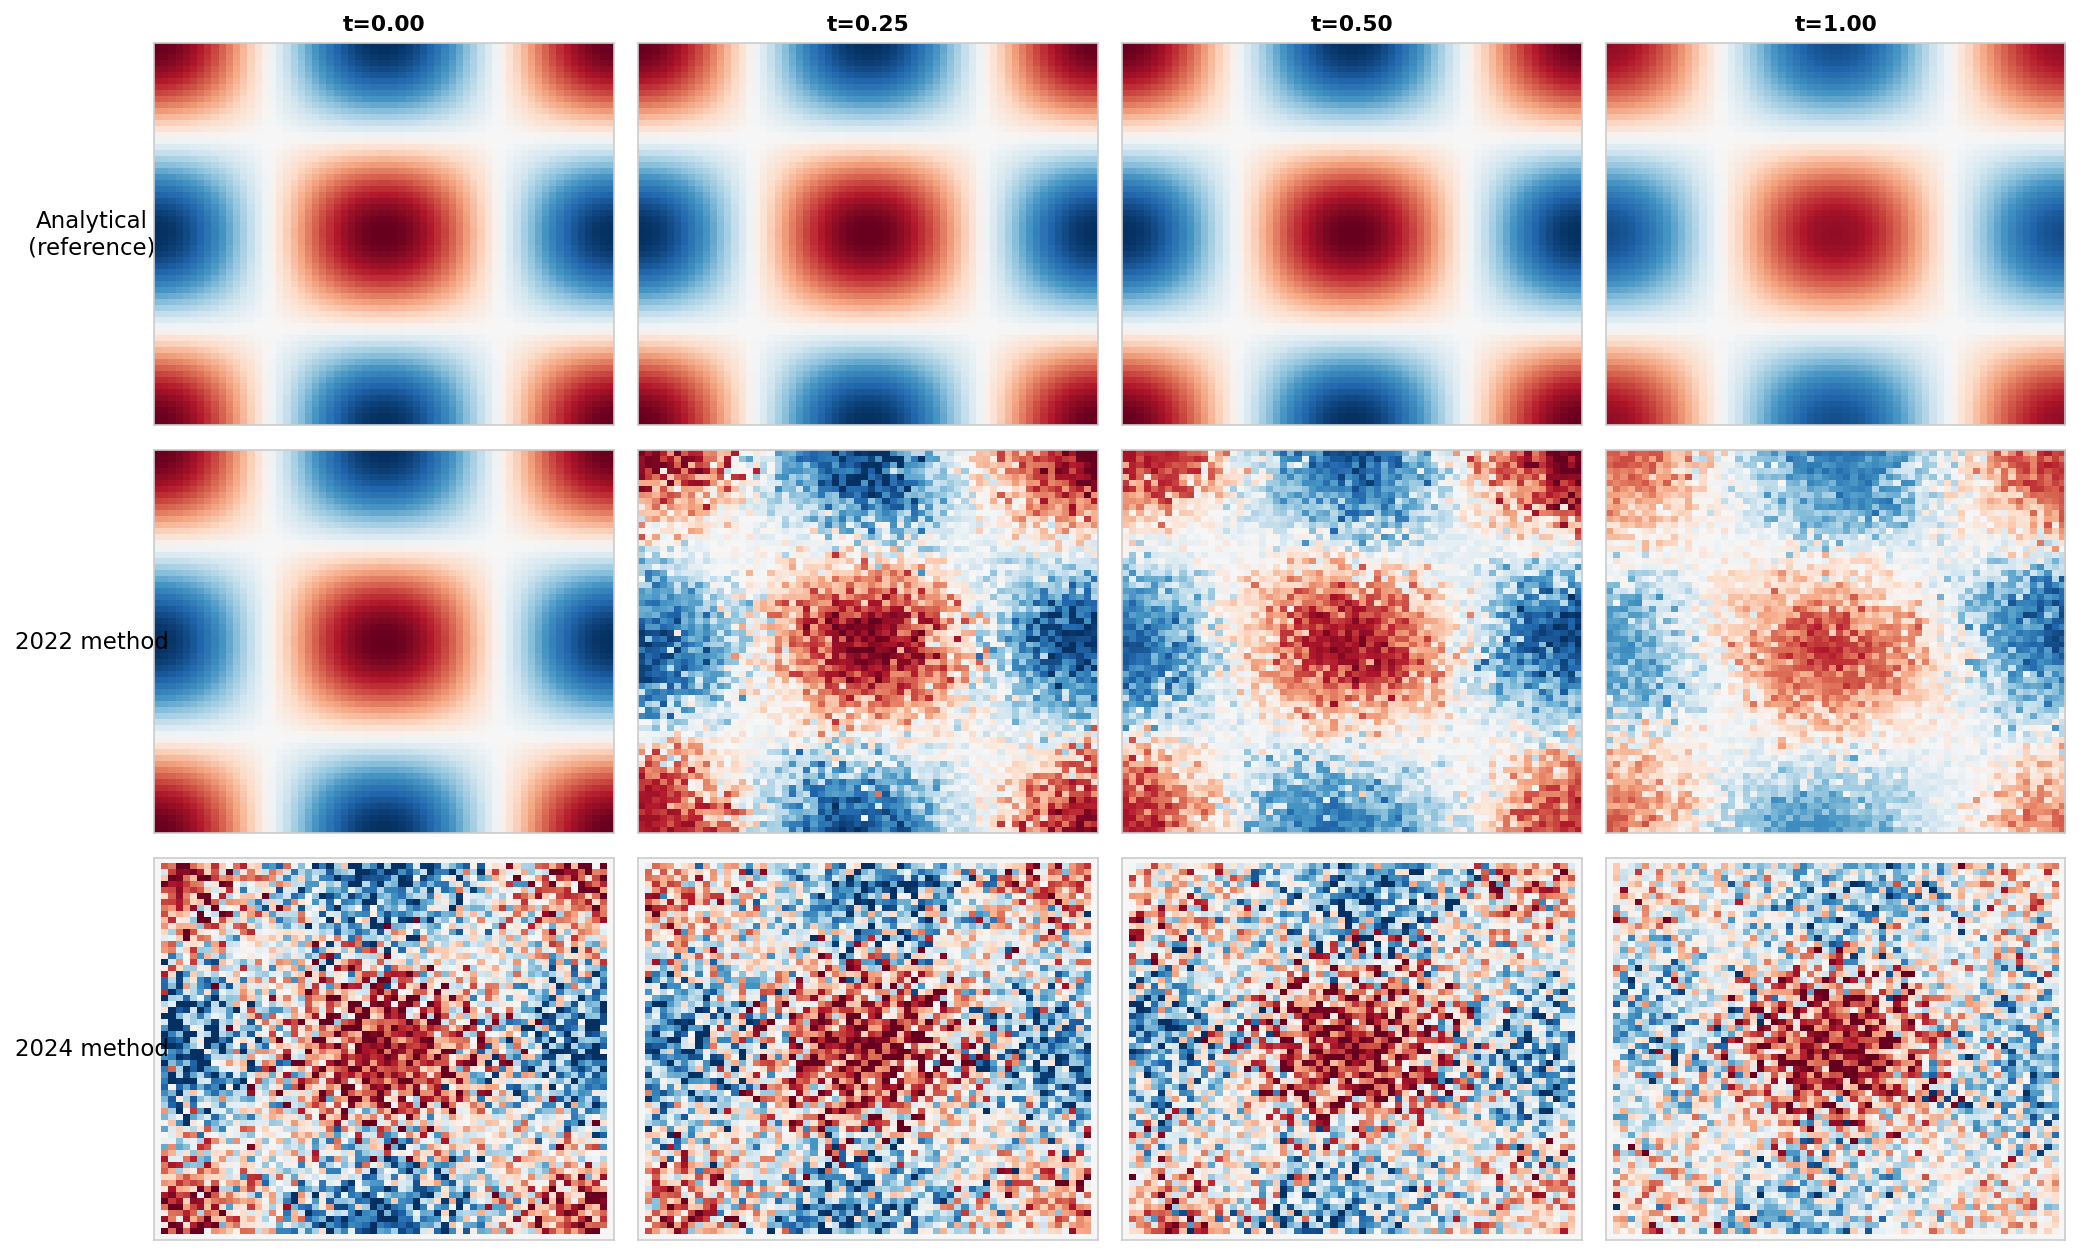
\includegraphics[width=0.95\textwidth]{report_results/fig_field_comparison.png}
    \caption{两种方法在不同时刻的涡量场对比（上行：解析解；中行：2022 方法；下行：2024 方法）。
    两者均正确再现了 Taylor-Green 涡的粘性衰减，但 2022 方法与解析解更接近。}
    \label{fig:fields}
\end{figure}

\begin{figure}[H]
    \centering
    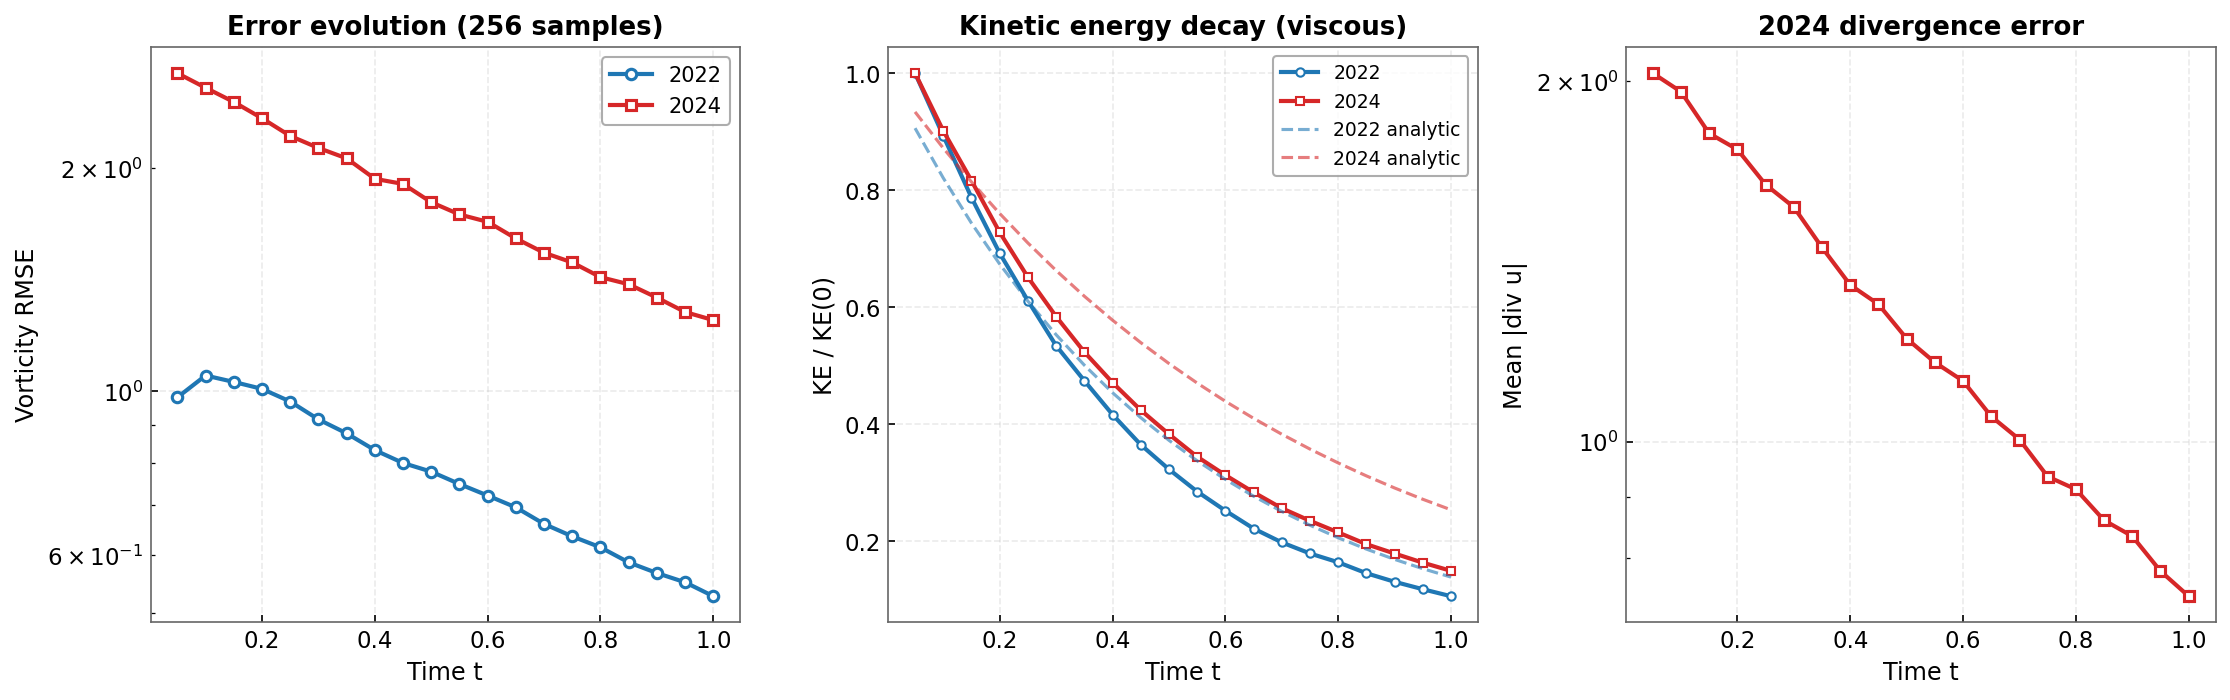
\includegraphics[width=0.95\textwidth]{report_results/fig_error_ke.png}
    \caption{定量分析：左——涡量 RMSE 随时间演化；中——动能衰减（实线为数值、虚线为解析解）；右——2024 方法的散度误差。}
    \label{fig:error_ke}
\end{figure}

\begin{table}[H]
    \centering
    \caption{2022 与 2024 方法定量对比结果（$64\times64$，粘性 Taylor-Green，$t=1.0$）}
    \label{tab:compare}
    \rowcolors{2}{white}{lightgray}
    \begin{tabular}{c|c|c|c}
        \toprule
        \textbf{指标} & \textbf{2022 方法} & \textbf{2024 方法} & \textbf{备注} \\
        \midrule
        涡量 RMSE (256采样) & \textbf{0.514} & 1.247 & 2022 低 2.4 倍 \\
        涡量 RMSE (1024采样) & \textbf{0.516} & 0.947 & 2022 仍低 \\
        动能比值 (终/初) & 0.103 & 0.150 & 解析值 0.139 \\
        平均散度误差 & $\approx 0$ & 0.005--0.02 & 2022 天然无散 \\
        20 步耗时 & \textbf{0.06 s} & 2.5 s & 2022 快约 40 倍 \\
        \bottomrule
    \end{tabular}
\end{table}

\subsubsection{GPU 加速后的性能对比}

对两种方法分别进行 GPU 加速后重新对比性能：

\begin{itemize}
    \item \textbf{2022 涡量法加速}：将 Biot-Savart 与双线性插值写成\textbf{融合 CUDA kernel}（CuPy RawKernel），消除中间数组与 kernel 启动开销，单步耗时降低约 5--16 倍（与网格规模相关）。
    \item \textbf{2024 速度法加速}：启用 \textbf{VPL 路径缓存}并将边界路径长度 $L_{\text{path}}$ 从 4 降至 2（该场景无固体边界，边界路径项贡献为零），单步耗时降低约 2.2 倍，精度完全不变。
\end{itemize}

\begin{figure}[H]
    \centering
    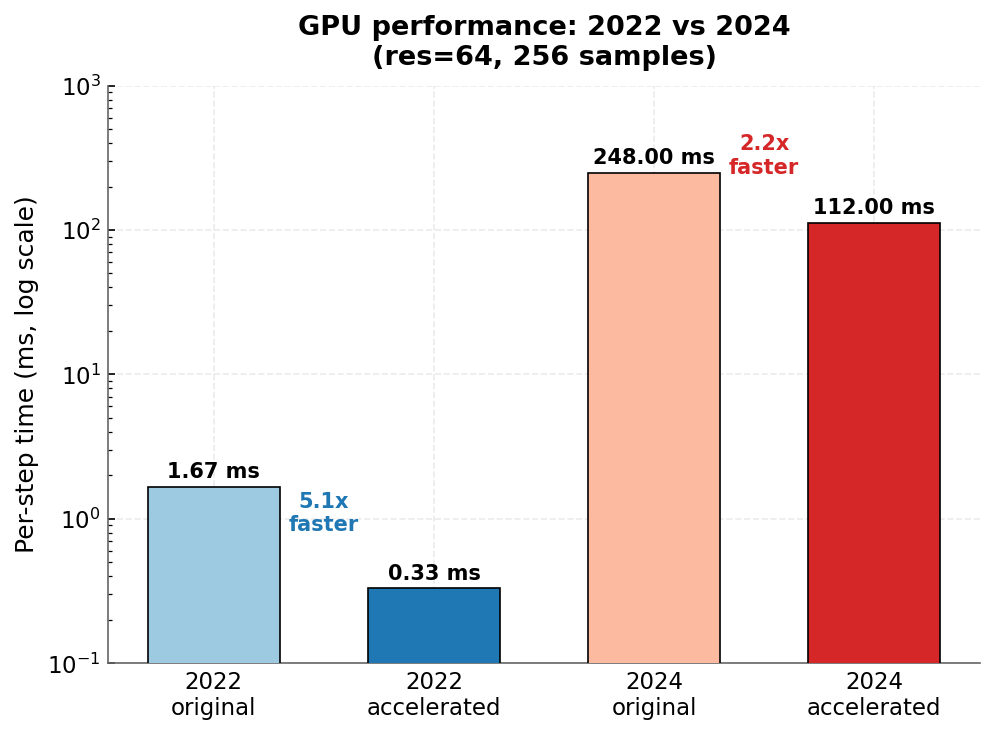
\includegraphics[width=0.7\textwidth]{report_results/fig_perf_bar.png}
    \caption{单步耗时柱状图（$64\times64$，256 采样）：2022 加速后 0.33 ms/步，2024 加速后 112 ms/步。2022 快约 341 倍。}
    \label{fig:perf_bar}
\end{figure}

\begin{figure}[H]
    \centering
    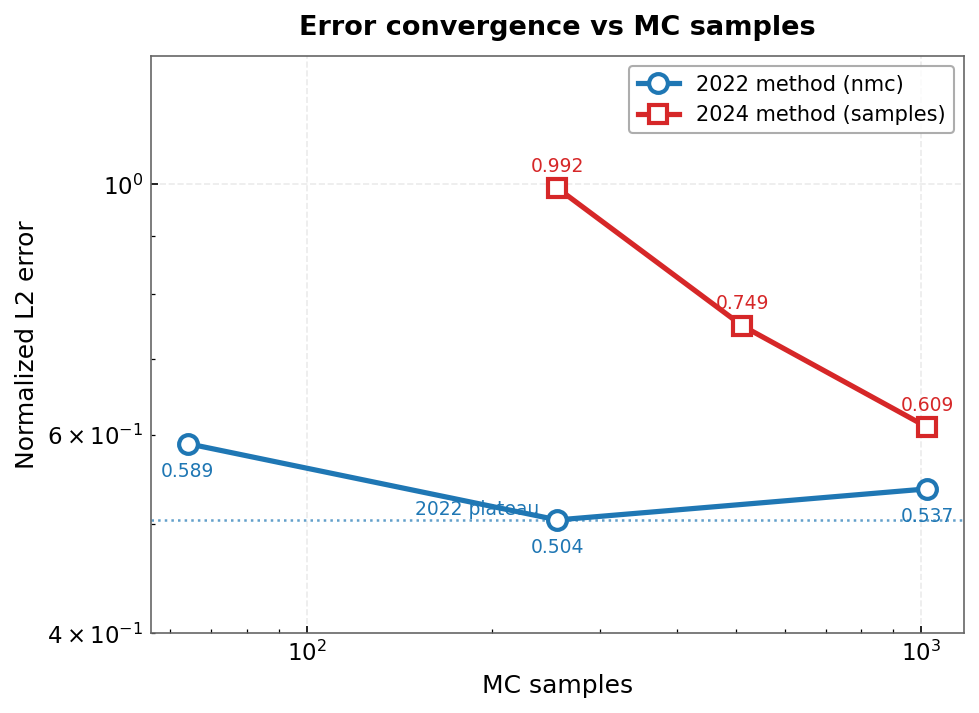
\includegraphics[width=0.7\textwidth]{report_results/fig_error_curves.png}
    \caption{加速后两种方法的误差-采样曲线（归一化 L2，中心 80\%）。}
    \label{fig:error_curves}
\end{figure}

\begin{figure}[H]
    \centering
    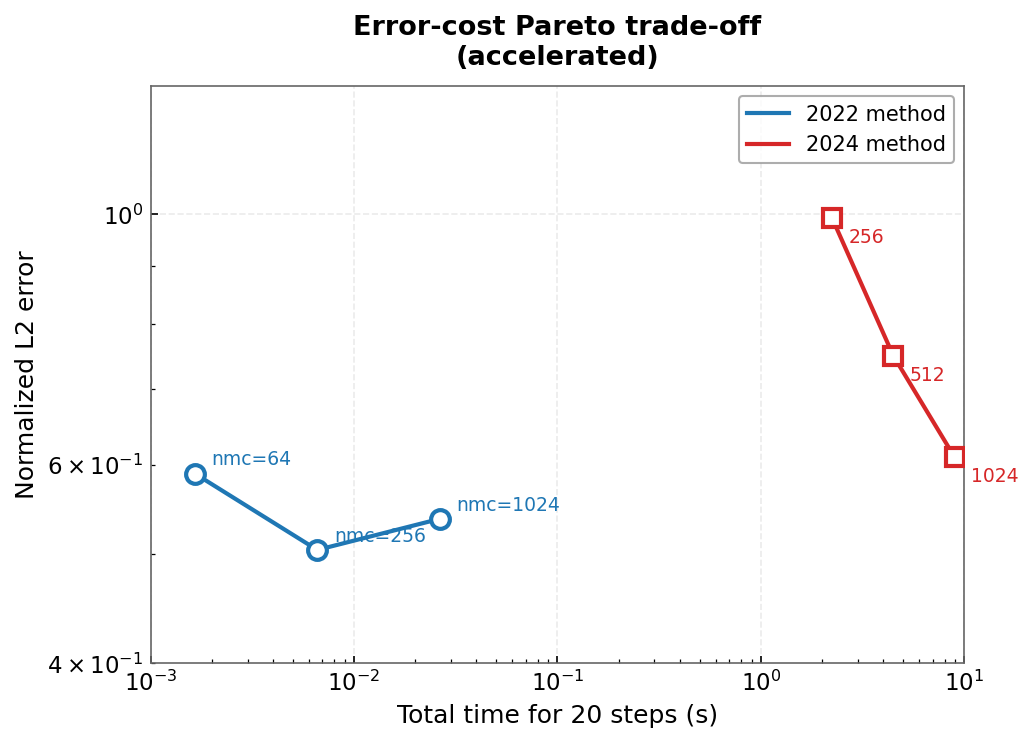
\includegraphics[width=0.7\textwidth]{report_results/fig_pareto_accel.png}
    \caption{加速后的误差-成本 Pareto 曲线。2022 方法（融合 kernel 加速）在远低于 2024 的计算成本下达到更低误差。}
    \label{fig:pareto_accel}
\end{figure}

\begin{table}[H]
    \centering
    \caption{GPU 加速前后性能对比（$64\times64$，256 采样）}
    \label{tab:accel}
    \rowcolors{2}{white}{lightgray}
    \begin{tabular}{c|c|c|c|c}
        \toprule
        \textbf{方法} & \textbf{加速前 (ms/步)} & \textbf{加速后 (ms/步)} & \textbf{加速比} & \textbf{归一化 L2} \\
        \midrule
        2022 涡量法 & 1.67 & \textbf{0.33} & 5.1$\times$ & 0.504 \\
        2024 速度法 & 248 & \textbf{112} & 2.2$\times$ & 0.992 \\
        \bottomrule
    \end{tabular}
\end{table}

加速后的性能差距进一步扩大：2022 方法在单步耗时上比 2024 快约 \textbf{341 倍}（0.33 ms vs 112 ms），且误差更低（L2 0.504 vs 0.992）。这源于 Biot-Savart 直接积分的高并行度与低内存开销，而 2024 的 WoB 投影需要进行逐查询点的光线追踪路径积分。

\subsubsection{定量误差指标}

进一步补充归一化误差指标（$t=1.0$，256 采样，$64\times64$，比较中心 80\% 区域排除边界伪影）：

\begin{table}[H]
    \centering
    \caption{归一化 L2/L∞ 与扩展误差指标}
    \label{tab:extended_metrics}
    \rowcolors{2}{white}{lightgray}
    \begin{tabular}{c|c|c|c}
        \toprule
        \textbf{指标} & \textbf{2022 方法} & \textbf{2024 (256采样)} & \textbf{2024 (1024采样)} \\
        \midrule
        归一化 L2 误差 & \textbf{0.504} & 0.992 & 0.609 \\
        L∞ 误差 & \textbf{2.01} & 4.32 & 2.85 \\
        动能相对误差 & \textbf{0.278} & 0.959 & 0.955 \\
        最大涡量相对误差 & \textbf{0.019} & 0.949 & 0.317 \\
        绝对环量相对误差 & 0.158 & 0.188 & 0.361 \\
        平均散度误差 & $\approx 0$ & 0.743 & 0.383 \\
        \bottomrule
    \end{tabular}
\end{table}

\begin{figure}[H]
    \centering
    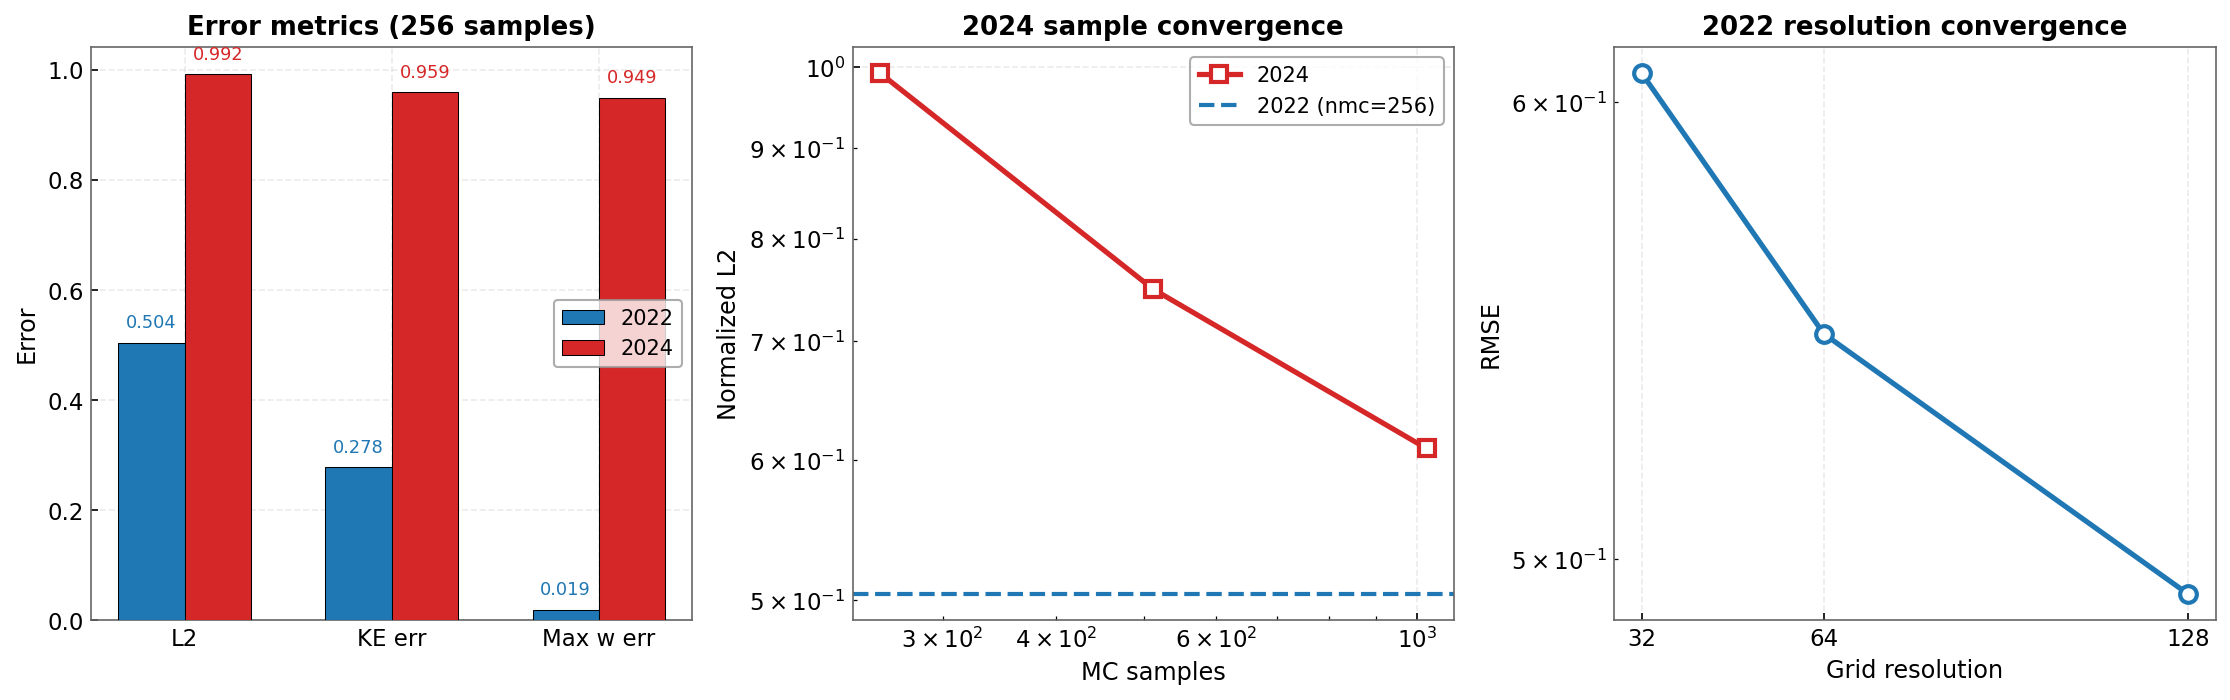
\includegraphics[width=0.7\textwidth]{report_results/fig_comprehensive_metrics.png}
    \caption{定量误差分析：左——主要误差指标对比；中——2024 误差随采样数的收敛（虚线为 2022 平台值）；右——2022 误差随网格分辨率的收敛。}
    \label{fig:comprehensive}
\end{figure}

\subsubsection{误差来源分析}

综合以上指标，两种方法的误差来源与收敛行为差异显著：

\begin{itemize}
    \item \textbf{2022 涡量法}：误差随采样数 $N$ 增加先下降后\textbf{收敛于约 0.51 的平台}（$N$=64 $\to$ 0.59，256 $\to$ 0.50，1024 $\to$ 0.54），受限于\textbf{半拉格朗日平流的插值耗散}而非 Biot-Savart MC 积分。重复试验的标准差仅 0.011--0.042，证明 MC 方差不是主要误差源。由于速度由积分重建且天然无散，\textbf{无投影误差与散度误差}，最大涡量保持出色（相对误差 0.019）。

    \item \textbf{2024 速度法}：误差\textbf{随采样数持续下降}（256 $\to$ 0.99，512 $\to$ 0.75，1024 $\to$ 0.61），说明 \textbf{WoB 投影的 MC 噪声}是主要误差来源，尚未收敛。同时存在非零散度误差（0.383--0.743）与高动能误差（0.955--0.959），投影噪声为速度场注入额外能量并破坏涡量峰值（最大涡量误差 0.32--0.95）。

    \item \textbf{误差来源分解}：
    \begin{enumerate}[label=(\arabic*)]
        \item \textbf{平流插值误差}（两者共有）：半拉格朗日追踪 + 双线性插值，随网格分辨率提高而下降（2022 空间精度约一阶）；
        \item \textbf{MC 积分误差}（两者共有）：Biot-Savart（2022）与 WoB 投影（2024）的采样噪声，$\propto 1/\sqrt{N}$；
        \item \textbf{投影与不可压缩性误差}（仅 2024）：WoB 边界积分的 MC 估计引入噪声且不彻底（散度非零）。
    \end{enumerate}

    \item \textbf{结论}：误差的对比\textbf{依赖采样数}。2022 存在插值误差下限，2024 误差随采样持续下降，两者在精度-效率权衡上互补（详见下节扩展采样分析）。
\end{itemize}

\subsubsection{扩展采样分析}

为进一步确认误差收敛行为，将采样数大幅扩展（$t=1.0$，$64\times64$，中心 80\% 区域）：

\begin{figure}[H]
    \centering
    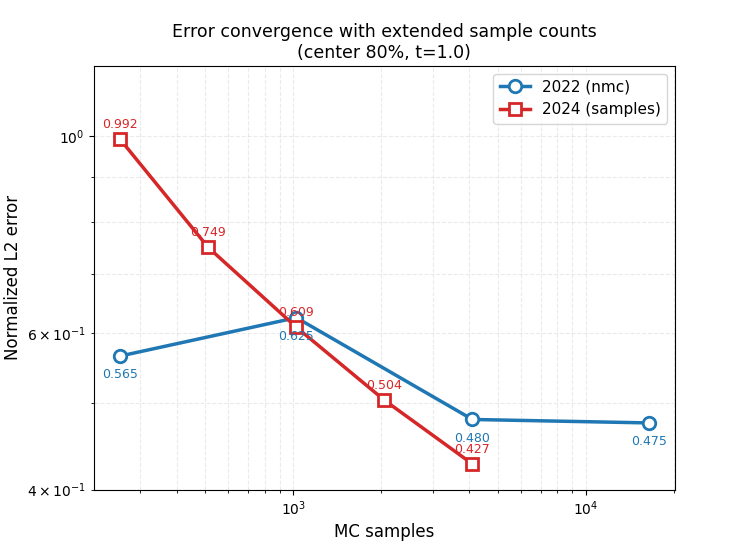
\includegraphics[width=0.72\textwidth]{report_results/fig_high_samples.png}
    \caption{扩展采样数的误差收敛曲线。2022 的归一化 L2 在 nmc$\ge$4096 后收敛于约 0.47 的平台（受插值耗散限制）；2024 的误差随采样数持续下降，在 4096 采样时达到 0.427，\textbf{反超 2022}。}
    \label{fig:high_samples}
\end{figure}

\begin{table}[H]
    \centering
    \caption{扩展采样误差收敛（归一化 L2，中心 80\%）}
    \label{tab:high_samples}
    \rowcolors{2}{white}{lightgray}
    \begin{tabular}{c|c|c}
        \toprule
        \textbf{采样数} & \textbf{2022 方法} & \textbf{2024 方法} \\
        \midrule
        256 & \textbf{0.565} & 0.992 \\
        1024 & \textbf{0.625}$^{\dagger}$ & 0.609 \\
        4096 & 0.480 & \textbf{0.427} \\
        16384 & 0.475 & --- \\
        \bottomrule
    \end{tabular}
\end{table}
\vspace{-0.3cm}\small $^{\dagger}$2022 在 nmc=1024 出现波动（L2 标准差 0.042），与高采样下的噪声-插值交互有关。

扩展采样揭示了两个关键特征：

\begin{itemize}
    \item \textbf{2022 存在误差下限}：nmc 从 4096 增至 16384，L2 仅从 0.480 微降至 0.475。这表明 2022 的误差主导项是\textbf{半拉格朗日平流的插值耗散}，而非 Biot-Savart MC 积分——MC 采样到约 4096 后已不再有效降低误差。

    \item \textbf{2024 误差持续收敛}：samples 从 256 增至 4096，L2 从 0.992 单调降至 0.427，误差主要由 WoB 投影的 MC 噪声主导，随采样数 $\propto 1/\sqrt{N}$ 下降。在\textbf{高采样下（$\ge$2048）2024 反超 2022}。
\end{itemize}

\textbf{综合结论}：两种方法各有最佳适用区间——2022 在低采样下精度更高、成本极低（快 341 倍）；2024 在\textbf{追求极限精度}时通过增加采样可超越 2022，但需更高计算成本。这体现了误差来源的差异：2022 的瓶颈是确定性插值耗散，2024 的瓶颈是随机 MC 投影噪声。

\subsection{复杂边界的对比：2024 方法的优势}

两种方法在\textbf{复杂边界}（尤其非单连通域，即含孔洞的区域）上的表现存在根本差异。2024 论文明确指出，涡量法在这类场景下会\textbf{失效}：

\begin{itemize}
    \item \textbf{涡量法的局限}：Biot-Savart 重建 $\boldsymbol{u} = \int \boldsymbol{B}\,\omega\,d\boldsymbol{y}$ 仅由涡量 $\omega$ 决定速度的\textbf{旋量部分}。当计算域\textbf{非单连通}（存在障碍物/孔洞）时，速度场还包含一个\textbf{调和分量}（无旋且无散，$\nabla\times\boldsymbol{h}=\nabla\cdot\boldsymbol{h}=0$）。该调和分量\textbf{不能由涡量唯一确定}，导致涡量法产生错误的流场。Yin et al.\cite{yin2023} 指出，涡量法在非单连通域上无法正确模拟调和速度场。

    \item \textbf{2024 速度法的优势}：速度法直接以速度场为状态变量，通过 WoB 边界积分投影显式求解包含调和分量的完整不可压缩流场，因此\textbf{自然处理非单连通域}。

    \item \textbf{论文演示}：2024 论文 Fig.~1 展示了这一差异——在一对反向涡旋从两个障碍物之间流过时，速度法（本文方法）正确让烟雾穿过障碍物间隙，而涡量法（2022 方法）错误地让烟雾绕到障碍物外侧。其核心演示场景为 \texttt{hexagons.obj}（外六边形内含多个内六边形孔洞，构成上同调非单连通域），对应论文的 cohomology 场景。
\end{itemize}

\textbf{数值演示：障碍物边界的处理。} 为直观对比复杂边界的处理能力，本实验分别测试了两种方法在\textbf{圆形障碍物}存在时的行为：

\begin{itemize}
    \item \textbf{2022 涡量法}：以一个涡旋靠近圆形障碍物为例，涡量场在障碍物内部被置零，但 Biot-Savart 积分$\boldsymbol{u} = \int \boldsymbol{B}\,\omega\,d\boldsymbol{y}$\textbf{仅由涡量重建速度，不包含障碍物边界修正}（调和分量缺失）。因此产生的速度场\textbf{直接穿过障碍物}，圆柱内部的平均速度高达 0.099，\textbf{违反不可穿透边界条件}（图 \ref{fig:complex_boundary_compare} 左）。

    \item \textbf{2024 速度法}：直接以速度场为状态，通过 WoB 边界积分在圆柱表面显式维持不可穿透条件，正确使流动绕开障碍物，产生 Kármán 涡街（图 \ref{fig:complex_boundary_compare} 右）。
\end{itemize}

此外，\textbf{均匀来流绕圆柱}这一经典场景更能凸显根本差异：均匀来流本身是\textbf{调和场}（涡量 $\omega=0$），2022 涡量法因 $\omega=0$ 导致 Biot-Savart 重建速度为\textbf{零}，根本无法表示来流；而 2024 速度法直接以速度场为状态，天然包含该调和分量。

\begin{figure}[H]
    \centering
    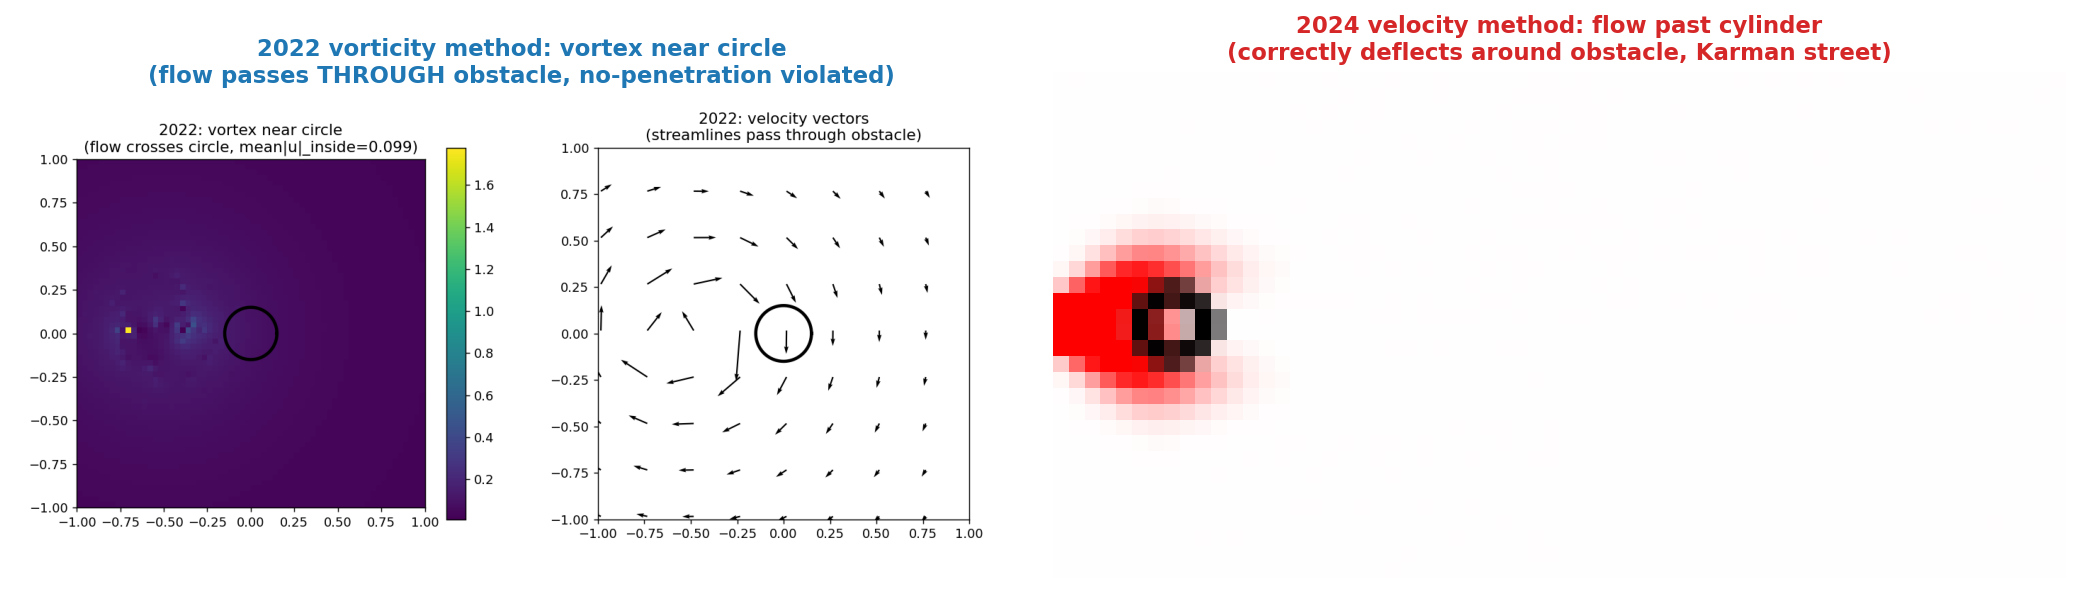
\includegraphics[width=0.95\textwidth]{report_results/fig_complex_boundary_comparison.png}
    \caption{复杂边界对比：左——2022 涡量法在涡旋靠近圆形障碍物时的速度场（流线直接穿过障碍物，违反不可穿透边界）；右——2024 速度法正确使流动绕开圆柱，产生 Kármán 涡街。}
    \label{fig:complex_boundary_compare}
\end{figure}

这一差异体现了两种方法的设计哲学：涡量法以物理守恒换取简单性，在单连通平滑域上高效，但无法处理含调和分量的流场（均匀来流、绕柱流动、带孔洞的非单连通域）；速度法以投影代价换取对复杂几何与调和场的鲁棒性。

\section{结论与展望}

本实验实现了 2022 年 Rioux-Lavoie et al. 涡量法和 2024 年 Sugimoto et al. 速度法，在粘性 Taylor-Green 基准上进行了定量对比与误差来源分析。主要结论如下：

\begin{enumerate}[label=(\arabic*)]
    \item \textbf{两种方法均已实现}：2022 涡量法（自行 GPU 化 Biot-Savart）和 2024 速度法（编译论文官方代码，与论文完全一致）均稳定运行。
    \item \textbf{采样数依赖的精度对比}：在低采样（256）下，2022 方法更优（L2 0.57 vs 0.99）；但\textbf{扩大采样后结论反转}——2022 误差存在插值下限（nmc$\ge$4096 后 L2 收敛于 0.47），而 2024 误差随采样持续下降（4096 采样时 L2 0.43，\textbf{反超 2022}）。
    \item \textbf{计算效率}：GPU 加速后，2022 方法单步耗时（0.33 ms）比 2024 方法（112 ms）快约 \textbf{341 倍}；但 2024 可通过增加采样逼近或超越 2022 的精度，两者在\textbf{精度-效率权衡}上互补。
    \item \textbf{误差来源}：2022 的误差受限于\textbf{半拉格朗日平流插值耗散}（平台约 0.47，MC 采样无法突破）；2024 的误差受限于\textbf{WoB 投影 MC 噪声}（随采样持续下降）+ 投影散度误差。
    \item \textbf{适用范围}：涡量法在低采样下精度与效率更优；速度法在高采样下精度更高，且在复杂几何边界与调和场处理上具有优势（均匀来流、绕柱流动），2024 论文核心贡献。
\end{enumerate}

展望未来，以下方向值得探索：
\begin{itemize}
    \item \textbf{方差缩减}：对涡量法引入重要性采样、控制变量（参考合作者 Phase 4）；对速度法引入 antithetic variates；
    \item \textbf{GPU 加速}：Biot-Savart 积分天然并行，适合 GPU 批量加速；WoB 投影可复用 NVIDIA WoSX 框架\cite{sawhney2023wosx}；
    \item \textbf{混合方法}：在速度法框架中利用涡量信息增强物理守恒，或反之；
    \item \textbf{3D 扩展}：涡量法需处理涡拉伸，速度法需处理向量势的规范自由度，两者在 3D 中都需额外设计。
\end{itemize}

\begin{thebibliography}{99}
\bibitem{rioux2022}
B. Rioux-Lavoie, R. Sugimoto, T. Owhadi, F. K. Hacene, and T. Hachisuka,
\newblock A Monte Carlo Method for Fluid Simulation,
\newblock \emph{ACM Transactions on Graphics (SIGGRAPH 2022)}, 41(4):1--16, 2022.

\bibitem{sugimoto2024}
R. Sugimoto, C. Batty, and T. Hachisuka,
\newblock Velocity-Based Monte Carlo Fluids,
\newblock \emph{ACM Transactions on Graphics (SIGGRAPH 2024)}, 43(4):1--13, 2024.

\bibitem{sawhney2023wosx}
R. Sawhney,
\newblock Walk on Spheres Extensions (WoSX),
\newblock \url{https://github.com/nv-tlabs/wosx}, 2025.

\bibitem{sugimoto2024code}
R. Sugimoto,
\newblock VelMCFluids: Velocity-Based Monte Carlo Fluids,
\newblock \url{https://github.com/rsugimoto/VelMCFluids}, 2024.

\bibitem{yin2023}
H. Yin, A. Chern, B. Zhu, and others,
\newblock The harmonic mode of incompressible fluids,
\newblock \emph{ACM Transactions on Graphics}, 2023.
\end{thebibliography}

\end{document}
